\chapter{Introduction}
\addcontentsline{toc}{chapter}{Introduction}
\markboth{Introduction}{Introduction}
\label{chap:introduction}
%\minitoc

%%% Local Variables: 
%%% mode: latex
%%% TeX-master: "isae-report-template"
%%% End: 

\section{D3S, a leader in 3D CAD Analytics}

D3S, which stands for Data Science Softwares \& Services, specializes in delivering customized software solutions utilizing AI technologies. The company comprises a team of Data Scientists and Full Stack Developers with deep expertise in 3D CAD (Computer-Aided Design) Analytics and Natural Language Processing (NLP).  

Its state-of-the-art technologies are built on open-source libraries and supported by internal R\&D, enabling efficient data extraction through computer vision, Optical Character Recognition (OCR), and NLP. D3S also excels in deep learning applications such as 3D morpho analysis, metrics comparison, BoM (Bill of Materials) analytics, and time series processing. 

The company’s solutions are designed to provide scalable, adaptable, and secure business value for industries like aerospace and automotive.

\vspace{0.5cm}

I have been working with the 3D CAD Analytics team, where my focus was on developing a 3D similarity model designed to compare CAD models solely based on their geometric properties.

\begin{figure}[]
    \centering
    
\includegraphics[width=0.3\columnwidth]{images/d3s_logo.png}
    \caption{D3S, Data Science Softwares \& Services}
    \label{fig:d3s_logo}
\end{figure}

\section{3D similarity model}

3D model designers spend a significant amount of time searching for relevant information during the product design process, even though much of their work could be done by modifying existing Computer-Aided Design (CAD) models. As a result, the retrieval and reuse of CAD models are crucial in CAD model management. However, large CAD model repositories often require extensive categorization or organization of engineering data, making design reuse challenging. Traditionally, the classification and retrieval of 3D CAD models involved a manual process of labeling, which is time-consuming, prone to errors, and inefficient. This issue becomes even more pronounced when models are generated in product development, as inconsistent labeling and tagging across different systems lead to the complex task of data harmonization. Additionally, the inherent complexity of 3D CAD model definitions makes it difficult to apply rigid, general classification rules, as model features and parameters vary depending on their origin. Therefore, an automated approach to classification and retrieval is needed to address these challenges.

The goal is to automatically associate a given piece to similar other pieces, as depicted in \autoref{fig:similar-pieces}. This will make it possible to leverage the D3S dataset of industrial 3D models, in order to infer missing information, such as the name of a piece, its function, or its material.

\begin{figure}[]
    \centering
    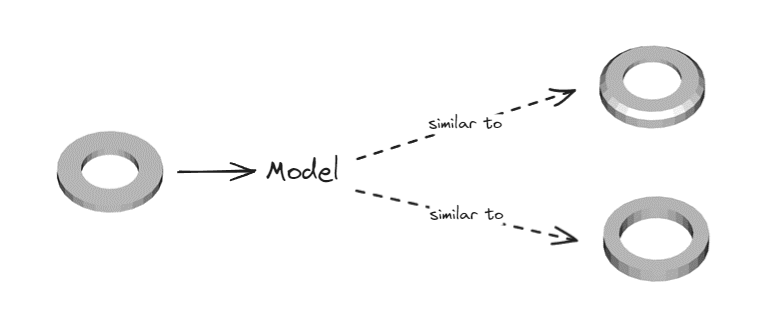
\includegraphics[width=0.8\columnwidth]{images/similar-pieces.png}
    \caption{Purpose of our similarity model}
    \label{fig:similar-pieces}
\end{figure}

In recent years, point cloud representations has become one of the research hotspots in the field of computer vision \cite{zhangDeepLearningbased3D2023}.
In our case, we can not directly train a powerful classifier, because of a lack of clean labeled data and of the variety of the possible 3D models.
The most comprehensive dataset available consists of just 2,000 CAD models, with rather imprecise labeling. Examples of labels include coupling strap, shackle, and long beam. It is evident that there is a significant need for a more curated and accurate dataset in this area, which is really hard to obtain.

Given the recent success of self-supervised learning methods, more specifically contrastive learning \cite{radfordLearningTransferableVisual2021,yuPointBERTPretraining3D2022,liuOpenShapeScaling3D2023}, an innovative and promising approach has been proposed to tackle this problem.

The goal is to learn a representation of data such that similar instances are close together in the representation space, while dissimilar instances are far apart. To do so, a triplet loss, popularized by the FaceNet model \cite{schroffFaceNetUnifiedEmbedding2015}, will be used. Since we lack labeled data, we can't generate triplets directly as in \cite{schroffFaceNetUnifiedEmbedding2015}. Instead, a 'Tinder-like' application has been developped and used by the whole company to build our labeled triplets database. To clarify, a labeled triplet consists of three 3D models: an anchor, a positive, and a negative model. The detailed framework of our triplet loss is outlined in \autoref{sec:triplet-loss-training}. In this setup, the anchor and positive models are similar to each other, whereas the negative model is distinct from both.

To summarize, the pipeline comprises the two main following steps:
\begin{enumerate}
    %TODO coherence with other sections
    \item \textbf{Triplets collection}: Offline unlabeled triplets are generated. Triplets are then labeled by the users of the app and stored in the database.
    \item \textbf{Model training}: An encoding model is trained on the labeled triplets. The model is then used to compute the similarity between two 3D models.
\end{enumerate}

\begin{figure}[]
    \centering
    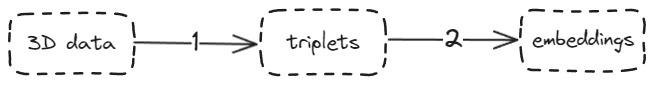
\includegraphics[width=0.8\columnwidth]{images/steps.png}
    \caption{Pipeline for building the model}   
    \label{fig:steps}
\end{figure}